\chapter{The Aegean Linear Scripts}
Linear A and Linear B were writing systems used during the Bronze Age, primarily on the island of Crete, with some discoveries also made on the Greek mainland.

\section{Historical Context}
Around 2000 BCE, the already established Minoan civilization on the island of Crete began constructing large, complex architectural buildings commonly referred to as "palaces."
These edifices served not only as administrative and economic centers, but also played important religious and ceremonial roles within Minoan society.

The founders of these palatial complexes were undoubtedly powerful landowners.
Minoan society was highly organized and capable of mobilizing substantial manpower for major construction projects, such as leveling the hilltops at Knossos and Phaistos and erecting monumental palaces. \cite{alexiou-ch2}

Hence, this highly structured society began to feel the need for a form of administrative writing to record transactions, compile inventories, and manage other aspects of economic and bureaucratic activity.

The first form of writing developed by this society was a logographic script known as Minoan Hieroglyphics, or Cretan Hieroglyphics, attested between 2100 and 1700 BCE.
The earliest and most archaic script was composed entirely of logographic symbols, which superficially resembled Egyptian hieroglyphs.
It was later abandoned in favor of a linear script known as Linear A, employed between 1800 and 1450 BCE.
The two systems initially coexisted for over a century, but in the following years, Linear A gradually replaced the former and became the sole writing system in use. \cite{salg-ch1}

Notably, the latest attestations of Cretan Hieroglyphs date to around 1700 BCE, when a catastrophe struck the island of Crete.
All the palaces in the island's three main centers, Knossos, Phaistos, and Malia were destroyed.
However, this did not lead to a cultural shift, as the palaces were promptly rebuilt, marking the passage from the Proto-palatial to the Neo-Palatial phase in Minoan history. \cite{alexiou-ch3}

This second phase of palace construction is the one that has survived to the present day, particularly at sites such as Knossos, Phaistos, Malia, and Zakros.

In 1450 BCE, a major catastrophe struck, probably caused by the eruption of the Thera volcano.
It triggered devastating earthquakes and a tidal wave that swept the north coast of Crete.
As a result, the main centers of Minoan civilization, Phaistos, Aghia Triadha, Malia, the mansions of Tylissos and Ammisos, as well as the eastern cities of Gournia and Zakros, were reduced to ruins.
Knossos also suffered significant damage, often accompanied by widespread fires. \cite{alexiou-ch4}

In 1400 BCE, Crete began losing its central cultural role, and the focus shifted to mainland Greece, particularly the Peloponnese.
The palace of Knossos was destroyed, while major fortified citadels (fortresses) were built in places like Mycenae and Tiryns. \cite{alexiou-ch5}

During this period, a new linear writing system emerged.
Although visually similar to Linear A, it encoded a different language: an archaic form of Ancient Greek.
Its name is Linear B, and it was used from 1400 to around 1100 BCE on Crete and the Greek mainland.
The Mycenaean civilization, which flourished during this period, is characterized by its extensive use of Linear B for administrative purposes, particularly in palace economies.
However, the destruction in Crete should not be interpreted as a Mycenaean military takeover, but rather as a transformative phase of socio-political and cultural adaptation. \cite{salg-ch5}


\begin{table}[h!]
\centering
\caption{Chronological framework of LA and LB \cite{salg-ch1}}

\begingroup
\renewcommand{\arraystretch}{0.9}
\resizebox{\textwidth}{!}{%
\begin{tabular}{|c|c|c|c|c|c|c|}
\hline
\multicolumn{1}{|c|}{\textbf{Chronology}} & \multicolumn{3}{c|}{\textbf{Crete}} & \multicolumn{3}{c|}{\textbf{Mainland}} \\
\hline
\textbf{High Dating} & \textbf{Pottery Phase} & \textbf{Cultural Phase} & \textbf{Scripts} & \textbf{Pottery Phase} & \textbf{Cultural Phase} & \textbf{Scripts} \\
\hline
1900--1800 & MM II      & \multirow{2}{*}{Proto-Palatial} & CH; LA & MH III   & \multirow{2}{*}{--}               &  -- \\
1800--1700 & MM III     &                                & CH; LA & MH III   &                                 &  -- \\
\hline
1700--1600 & LM IA      & \multirow{2}{*}{Neo-Palatial}   & LA     & LH I     & \multirow{3}{*}{Early Mycenaean} & LA \\
1600--1450 & LM IB      &                                 & LA     & LH IIA   &                                 & ? \\
\cline{1-4}
1450--1400 & LM II      & \multirow{2}{*}{Final-Palatial} & LA?    & LH IIB   &                                 & ? \\
\cline{5-7}
1400--1375 & LM IIIA1   &                                 & LB     & LH IIIA1 & \multirow{4}{*}{Late Mycenaean}  & LB \\
\cline{1-4}
1375--1300 & LM IIIA2   & \multirow{3}{*}{Post-Palatial}  & LB     & LH IIIA2 &                                 & LB \\
 % separate lines for Crete and Mainland
1300--1200 & LM IIIB    &                                 & LB     & LH IIIB  &                                 & LB \\
% separate lines for Crete and Mainland
1200--1050 & LM IIIC    &                                 & --     & LH IIIC  &                                 & LB \\
\hline
\end{tabular}
}
\endgroup
\end{table}


\section{The main sites}
The main sites where Linear A documents have been found are located on the island of Crete. These include Knossos, Phaistos, Aghia Triada, Zakros, Khania, Tylissos, and Malia.

\begin{figure}[H]
    \centering
    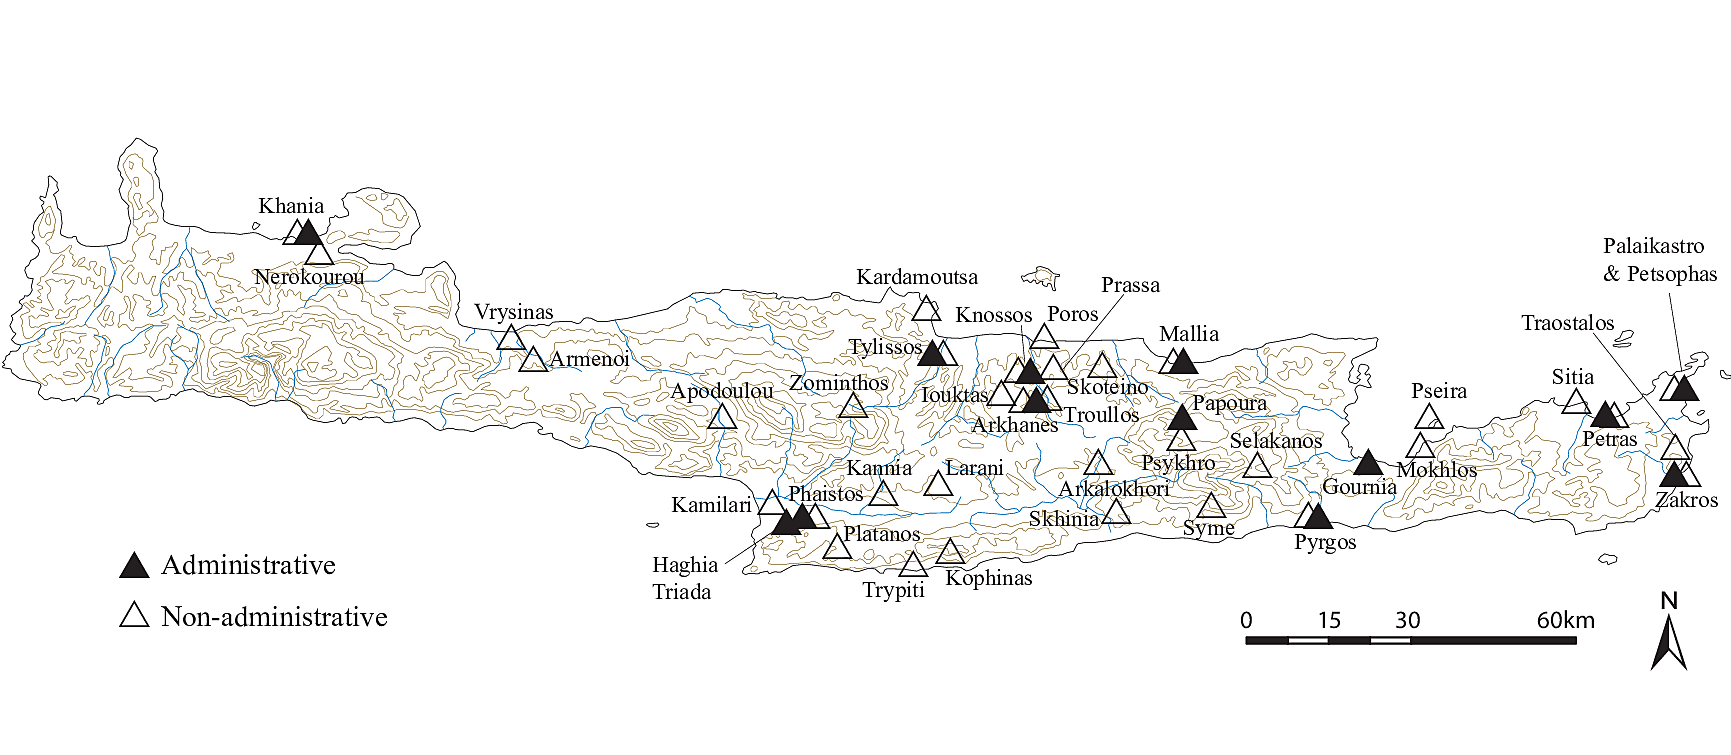
\includegraphics[width=0.8\textwidth]{Images/crete_LA.png} % Adjust width and filename
    \caption{Sites of Linear A fragments in Crete.\protect\footnotemark}
    \label{fig:crete_LA}
\end{figure}
\footnotetext{Figure \ref{fig:crete_LA} prepared by Yannis Galanakis and Ester Salgarella.}

Linear A was more widespread, covering completely Crete and the Aegean Islands and reaching the Greek mainland.
The main attestations of Linear A on the Greek mainland are very limited and generally considered sporadic and isolated. 
At Mycenae, a few Linear A inscriptions have been found, likely as a result of commercial or cultural exchanges with Crete. 
Similarly, some fragmentary finds have been uncovered at Tiryns, probably also related to trade or contacts with Minoan Crete.

\begin{figure}[H]
    \centering
    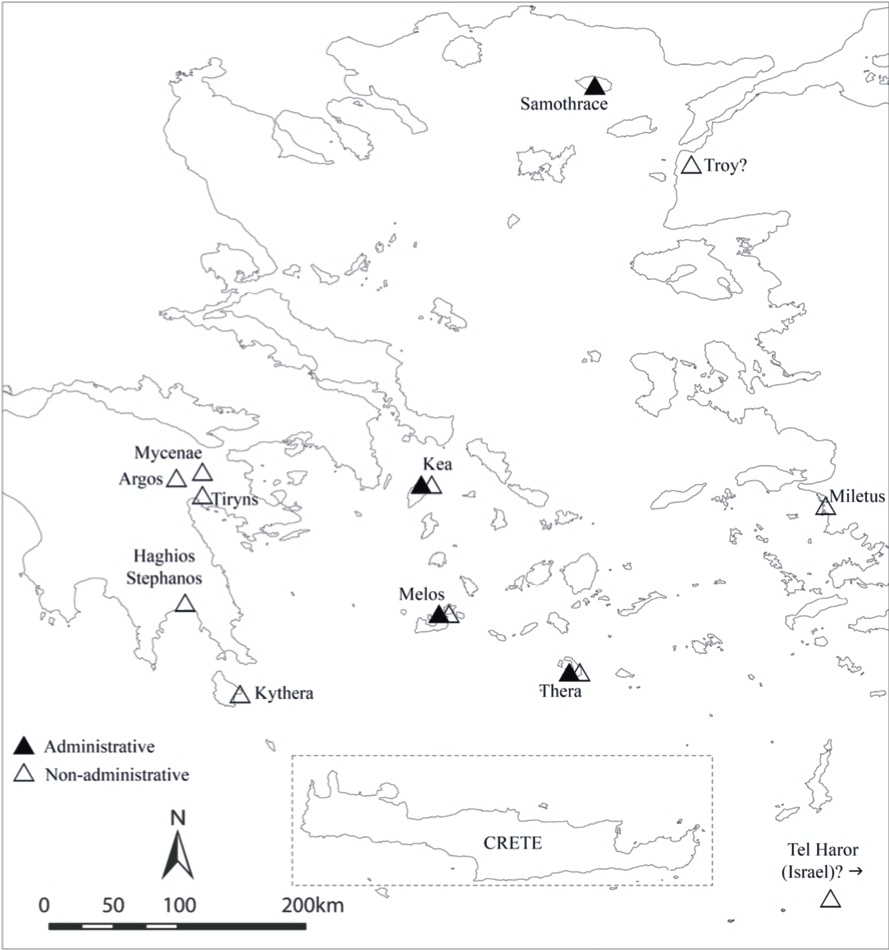
\includegraphics[width=0.8\textwidth]{Images/mainland_LA.jpg} % Adjust width and filename
    \caption{Sites of Linear A fragments in the Greek mainland.\protect\footnotemark}
    \label{fig:mainland_LA}
\end{figure}
\footnotetext{Figure \ref{fig:mainland_LA} prepared by Yannis Galanakis and Ester Salgarella.}

In contrast, Linear B is extensively attested on the Greek mainland, particularly in the Peloponnese, reflecting its administrative function during the Mycenaean period.
Major sites where Linear B documents have been found include Mycenae, Tiryns, Pylos, Thebes, and Athens.
Additionally, significant findings of Linear B tablets have been made in Crete, especially at Knossos and Khania.

The corpora of the two writing systems are relatively small, with Linear A consisting of approximately 1,400 documents, while Linear B comprises around 6,000 documents.
Another notable difference is that Linear A was more widely used for non-administrative purposes, particularly in religious contexts, whereas the number of non-administrative Linear B documents is considerably more limited. \cite{salg-ch1}


\begin{figure}[H]
    \centering
    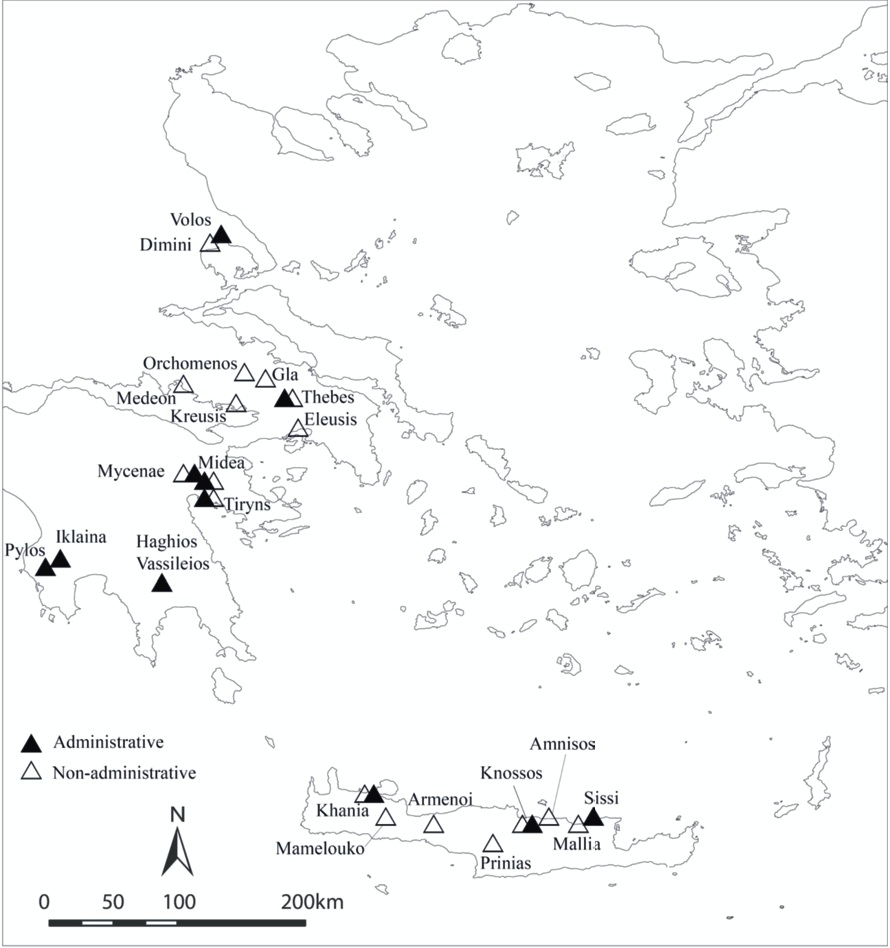
\includegraphics[width=0.8\textwidth]{Images/mainland_LB.jpg} % Adjust width and filename
    \caption{Sites of Linear B fragments in Crete and the Greek mainland.\protect\footnotemark}
    \label{fig:mainland_LB}
\end{figure}
\footnotetext{Figure \ref{fig:mainland_LB} prepared by Yannis Galanakis and Ester Salgarella.}


\section{Linguistic features}
The two writing systems are characterized by similar structural features, reflecting the connection between Linear A and Linear B and the derivation of the latter from the former.

The primary similarity between the two scripts lies in their syllabic structure, which constitutes a defining feature of both writing systems.
Both Linear A and Linear B are syllabic scripts, meaning that each symbol represents a syllable rather than an individual letter or a full word.
In addition to syllabic signs, both systems incorporate a set of logograms: symbols representing entire words or concepts.

This logographic component is particularly prominent in Linear A, where a significant number of signs are used to denote specific objects, actions, or concepts, often associated with administrative and religious contexts.
By contrast, Linear B employs a more restricted set of logograms, reflecting its primary function in administrative record-keeping.
Notably, the logograms used in Linear A were generally not inherited by Linear B, with a single exception: the logogram for "wool" (MA+RU), which is attested in both scripts.
However, the principles governing the formation of logograms remained unchanged, as in both scripts they are formed by juxtaposing or combining two or more signs, either horizontally or vertically.
\begin{figure}[H]
    \centering
    \begin{subfigure}[b]{0.6\textwidth}
        \centering
        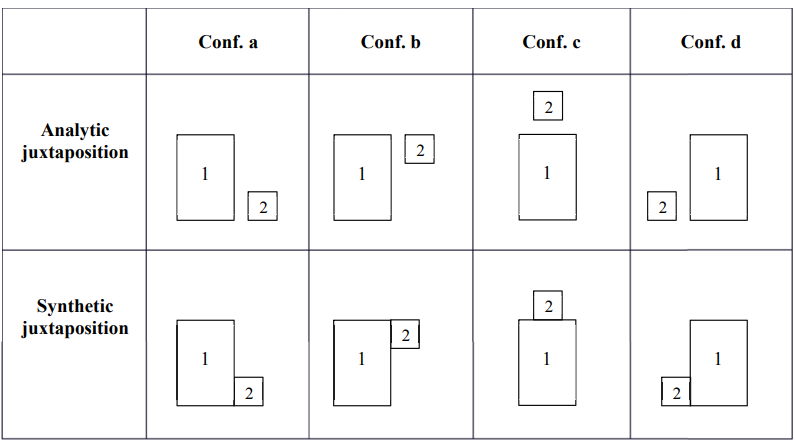
\includegraphics[width=\textwidth]{Images/logograms.png}
        \caption{Logogram construction criteria.}
        \label{fig:logograms}
    \end{subfigure}
    \hspace{0.05\textwidth}
    \begin{subfigure}[b]{0.3\textwidth}
        \centering
        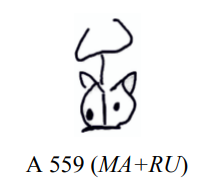
\includegraphics[width=\textwidth]{Images/ma-ru.png}
        \caption{LA logogram for wool.}
        \label{fig:ma-ru}
    \end{subfigure}
    \caption{Logograms in Linear A and Linear B.}
    \label{fig:linearA_sites}
\end{figure}

\begin{figure}[H]
    \centering
    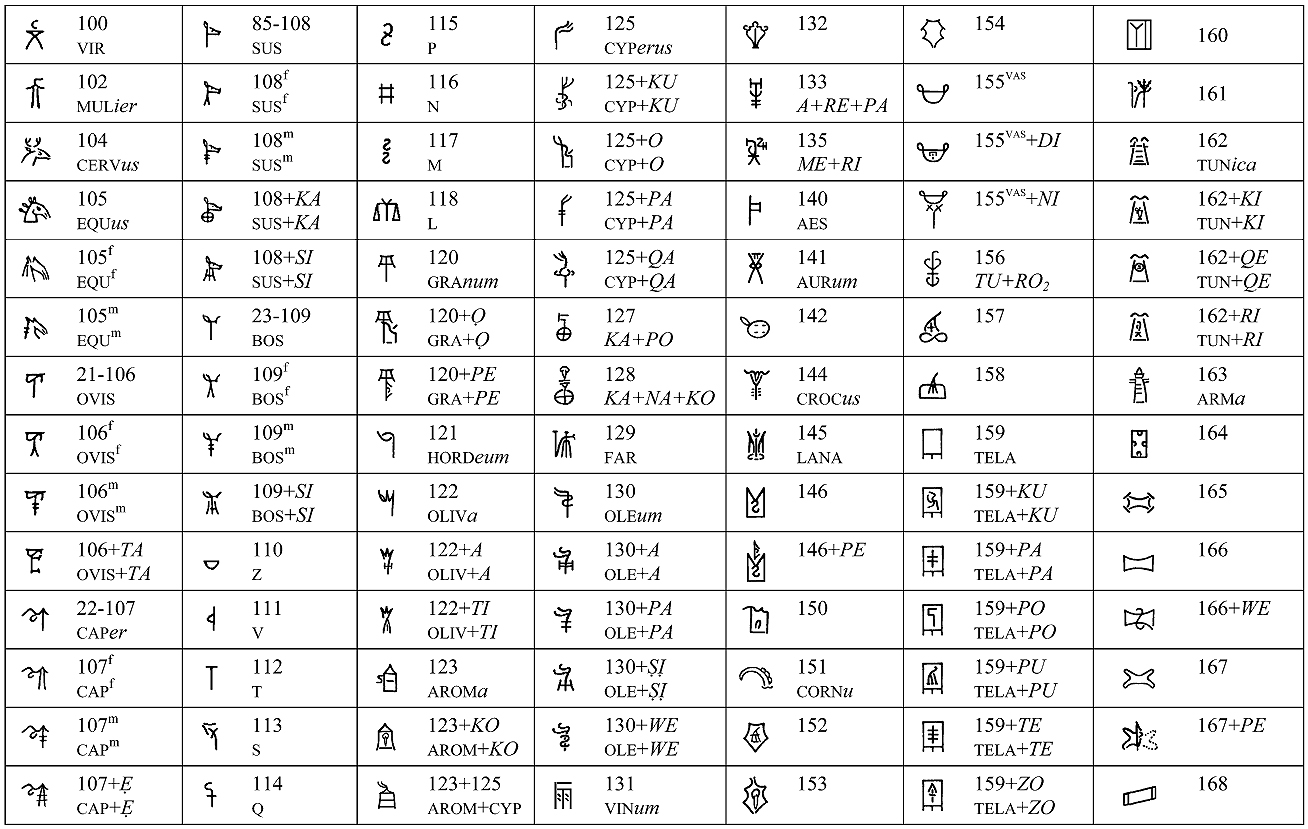
\includegraphics[width=1\textwidth]{Images/logos_1.jpg}
    \caption{Linear B logograms (symbols 100-168).}
    \label{fig:logos_1}
\end{figure}

Figure \ref{fig:logos_1} illustrates how logograms in Linear B can also incorporate syllabograms.
In these cases, the syllabogram is referred to as an adjunct and typically serves to qualify or specify the meaning of the logogram.
Moreover, the use of adjuncts is significantly more frequent in the Knossos corpus than on the Mainland, suggesting a possible continuity with Linear A, where isolated signs with sematographic value appear more commonly. \cite{salg-ch3}

Furthermore, a substantial portion of the Linear A syllabary is shared with Linear B, with approximately 72\% of Linear A signs being identical to those used in Linear B.
This overlap also illustrates continuity in symbol creation and in the assignment of phonetic values between the two systems.

\begin{figure}[H]
\centering
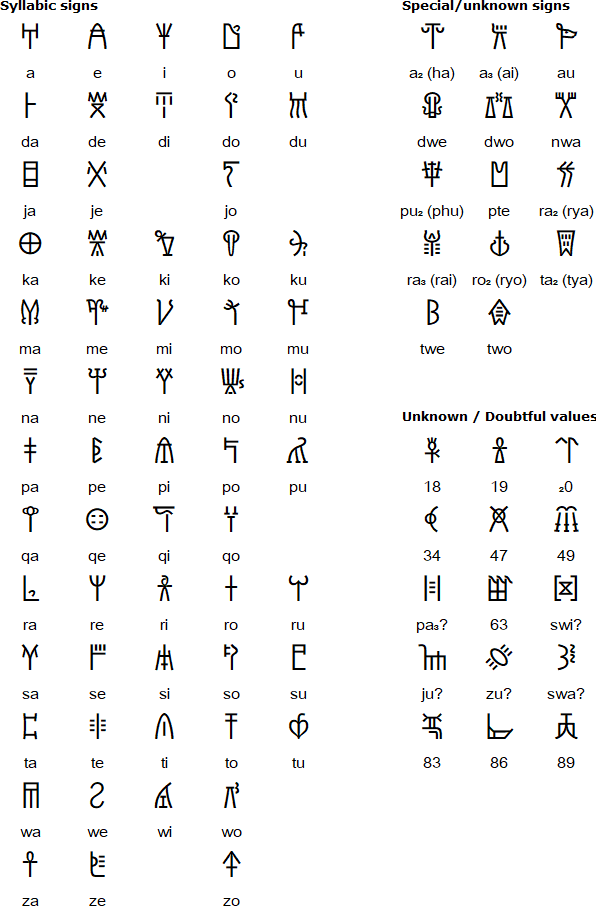
\includegraphics[width=0.8\textwidth]{Images/syll_LB.png}
\caption{All Linear B syllabograms with the associated phonetic values.}
\label{fig:syll_LB}
\end{figure}

As observed in Figure \ref{fig:syll_LB}, signs referring to the same vowel exhibit recurring patterns, a characteristic feature of syllabic scripts also evident in Linear A.
One of the most debated assumptions regarding the relationship between Linear A and Linear B is the principle of homomorphy and homophony.
This principle posits that signs which are visually similar (homomorphy) in both scripts also share the same phonetic value (homophony), representing the same syllable. \cite{salg-ch1}

This observation has led to the widely accepted conclusion that Linear A encodes a language fundamentally different from Linear B, with the latter used to represent an archaic form of Ancient Greek.
Consequently, although scholars are able to phonetically transcribe Linear A inscriptions, the language remains undeciphered and its meaning unknown. 

\section{The decipherment of Linear B} \label{sec:decipherment}
Ever since the discovery of the first Linear B tablets in 1900 by Sir Arthur Evans at Knossos, the script has been a subject of intense scholarly interest.
Evans himself introduced the classification of Aegean scripts that is still used today.
He also made the earliest attempts to decipher Linear B, though without success.

The breakthrough in understanding Linear B came after World War II, following major discoveries at the site of Pylos in 1939, which uncovered a large number of tablets and inscriptions.
A key figure in the decipherment of Linear B was Michael Ventris, a British architect and amateur linguist.
Ventris, in collaboration with philologist John Chadwick, succeeded in deciphering the script in 1952, demonstrating that it encoded an early form of Ancient Greek.

\subsection{The knowledge before the decipherment}

Before the decipherment of Linear B, scholars attempted to understand the script by studying it in isolation and by comparing it with known languages.  
One of the earliest hypotheses focused on the similarity between the Linear B syllabary and the Cypriot syllabary, a syllabic script used from about the eleventh to the fourth centuries BCE.  
The latter, which was also used to write an archaic form of Greek, shared a significant number of signs with Linear B.

However, this resemblance proved misleading in several respects.  
Although many signs appeared visually similar, as can be observed in Figure \ref{fig:lb-cypr}, their phonetic values often differed between the two systems.  
Moreover, the scripts treated grammatical suffixes differently.  
In Linear B, grammatical suffixes were frequently omitted, whereas this was not the case in the Cypriot syllabary, where the syllabogram "se" was regularly employed to indicate word endings.

Because "se" appeared regularly in the Cypriot syllabary but was rare in Linear B, early researchers concluded that Linear B could not represent the Greek language.  
In particular, Arthur Evans was convinced that the Minoan civilization was entirely distinct from the Mycenaean Greek world.  
This assumption, reinforced by Evans's authority and influence, contributed to delaying the recognition of the script's true linguistic nature. \cite{chad-ch2}

An example of this is the word "anthropos" (Ancient Greek: \textgreek{ἄνθρωπος}), which appears in Linear B as "a-to-ro-qo" (\textlinb{\Ba\Bto\Bro\Bqo}), while in Cypriot it is spelled with the "se" suffix as follows: "a-to-ro-po-se" (\textcypr{\Cse\Cpo\Cro\Cto\Ca}, written from right to left).

\begin{figure}[H]
\centering
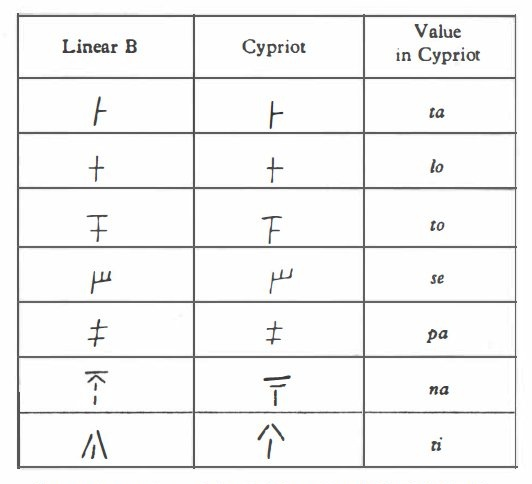
\includegraphics[width=0.6\textwidth]{Images/LB_cypriot.jpg}
\caption{Similarity between Linear B and Cypriot syllabary.}
\label{fig:lb-cypr}
\end{figure}

Evans had already established that most documents were administrative records.  
However, any attempt to decipher the script was hindered by unreliable underlying assumptions, while many aspects of the language remained unknown.

The most significant contribution came from Dr. Alice Kober, an American linguist. 
She was the first to approach the script methodically in order to uncover the nature of the underlying language.
She sought to answer fundamental questions, such as whether the language was inflected or whether specific forms were used to indicate gender and number.

Through her careful analysis, she was able to identify grammatical patterns, including distinctions between masculine and feminine nouns, as well as examples of inflection.
These results were achieved through a systematic study of repeated sign groups and their contexts, which she meticulously documented in her notebooks.
Her work challenged Evans's assumptions about the non-Greek nature of the language and paved the way for Ventris' later decipherment.
The outcome of her research was a set of "triplets", groups of three related words differing only in their endings, which provided critical evidence of an inflected language structure and were later referred to as "Kober's triplets".
Some examples of these triplets are shown in Figure \ref{fig:kobler_triplets}. \cite{chad-ch3}


\begin{figure}[H]
\centering
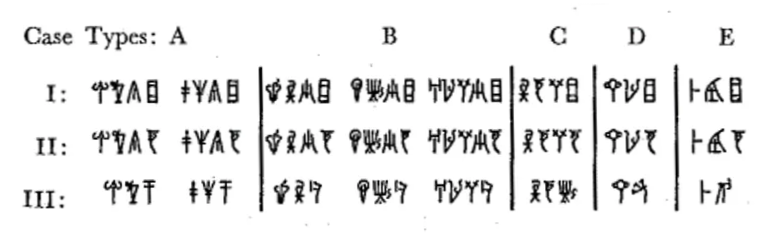
\includegraphics[width=0.8\textwidth]{Images/kobler_triplets.png}
\caption{Kobler's triplets examples.}
\label{fig:kobler_triplets}
\end{figure}

\subsection{The decipherment by Ventris and Chadwick} \label{subsec:ventris-chadwick}
The initial phase of the decipherment of Linear B involved the identification of numerical signs and easily recognizable logograms.
This preliminary work was largely accomplished by Sir Arthur Evans, who successfully identified the most frequently occurring logograms and reconstructed the basic features of the numerical system.
Notably, the Linear B script lacked a symbol for zero, but included fractional signs and was based on a decimal structure.

Building on these foundations, scholars began to assign tentative phonetic values to individual syllabograms through contextual analysis.
By examining recurring patterns and the placement of signs within administrative texts, it became possible to propose the phonetic values of certain symbols.
For instance, words such as "total" and "sons," which regularly appeared in similar tabular contexts, offered valuable clues for these early phonetic assignments.

However, the construction of a comprehensive and reliable grid of syllabograms was not feasible until the publication of the Pylos tablets in 1951.
This newly available corpus significantly expanded the body of evidence, enabling more systematic linguistic analysis.

Michael Ventris began his work on the decipherment in 1950, initially by circulating a questionnaire among scholars to gather views on the possible nature of the language encoded in Linear B and its potential relationship to Linear A or the Cypriot syllabary.

Realizing that scholarly opinion was divided, Ventris adopted a combinatorial and structural approach.
He explored positional patterns of signs within words, aiming to deduce their possible function or phonetic value.
By analyzing the frequency and distribution of certain symbols, particularly those likely to represent vowels, he was able to identify a subset of syllabograms corresponding to pure vowels.

A key breakthrough came from the identification of inflectional endings, many of which were made possible by the foundational work of Alice Kober.
Kober had demonstrated, through rigorous tabulation of sign groups, that the language encoded by Linear B exhibited an inflectional structure.
Ventris incorporated these findings into his research and began constructing a syllabic grid, updating it continually in light of new phonological rules and morphological patterns.

For example, he correctly identified the syllabogram \textlinb{\Bsi} as representing the syllable si, based on its frequent use in noun declensions and verb conjugations.
Its function mirrored that of the Ancient Greek suffix \textgreek{σι}, which appears in both oblique noun forms and verbal endings.

Additionally, place names proved particularly helpful, especially when accompanied by adjectival derivatives.
These offered valuable comparisons with known Greek toponyms and morphological structures.

As Ventris refined his hypotheses and incorporated increasingly sophisticated linguistic deductions, especially regarding inflectional patterns and suffixes, he was able to assign phonetic values to a majority of the signs.
Through this methodical approach, he successfully constructed a nearly complete syllabary grid.
Most of his assignments proved to be correct, with only minor exceptions that were later adjusted through collaborative efforts with John Chadwick and subsequent scholarly review. \cite{chad-ch4}

\begin{figure}[H]
\centering
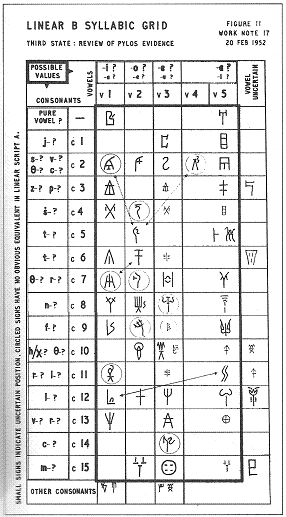
\includegraphics[width=0.8\textwidth]{Images/ventris_grid.png}
\caption{Ventris' syllabary grid.}
\label{fig:ventris_grid}
\end{figure}

Together, Ventris and Chadwick continued to investigate how the script encoded the phonology of the Mycenaean Greek language, recognizing that Linear B imposed structural constraints on how sounds were represented.
The syllabary, like many early writing systems, lacked a one-to-one correspondence with spoken Greek.
To better understand these adaptations, they analyzed the principles governing the script's orthography, namely how Greek words were transcribed within the limitations of the Linear B system.

The following rules summarize the most significant phonological and orthographic conventions that Ventris and Chadwick identified in the course of their research:

\begin{enumerate}
\item The script distinguishes five vowels: \textit{a, e, i, o, u}. Vowel length, however, is not indicated.

\item The second component of diphthongs ending in \textit{-u}, such as \textit{au, eu, ou}, is represented explicitly.

\item In diphthongs ending in \textit{-i} (e.g., \textit{ai, ei, oi, ui}), the second component is generally omitted, except:
\begin{itemize}
    \item when it occurs before another vowel, in which case it is represented as \textit{y};
    \item in the initial syllable \textit{ai}, where the full diphthong is retained.
\end{itemize}

\item Glides occurring between a front vowel and a following vowel are indicated:
\begin{itemize}
    \item the glide after \textit{i} is written as \textit{j};
    \item the glide after \textit{u} is written as \textit{w}.
\end{itemize}
These sounds are typically omitted in Greek alphabetic spelling.

\item The script represents twelve consonants:
\begin{itemize}
    \item \textbf{j}: used only to represent diphthongal \textit{i} or as a glide (see point 3);
    \item \textbf{w}: corresponding to the archaic Greek digamma (\textit{\textgreek{ϝ}}), pronounced as in English \textit{w};
    \item \textbf{d, m, n, s}: approximately as in later Greek and English;
    \item \textbf{r}: corresponding to Greek \textit{l} and \textit{r};
    \item \textbf{z}: corresponding to Greek \textit{z}; its exact phonetic value in Mycenaean Greek remains uncertain;
    \item \textbf{p, t, k}: representing both plain and aspirated stops, as the script does not distinguish aspiration;
    \item \textbf{q}: representing a series of labio-velar stops (\textit{kw, gw, khw}), which later disappeared from Greek but were preserved in Latin (e.g., \textit{quis}, \textit{unguem}).
\end{itemize}

\item The script does not represent aspiration; thus, aspirated consonants (\textit{ph, th, kh}) are not distinguished from their unaspirated counterparts.

\item The consonants \textit{l, m, n, r, s} are omitted when they occur:
\begin{itemize}
    \item at the end of a word;
    \item before another consonant.
\end{itemize}
For example, \textit{po-me} = \textit{poimen} (\textgreek{ποιμήν}) "shepherd"; \textit{ka-ko} = \textit{khalkos} (\textgreek{χαλκός}) "bronze"; \textit{pa-te} = \textit{pater} (\textgreek{πατήρ}) "father".

\item Initial \textit{s-} is generally omitted before another consonant.

\item In consonant clusters involving a stop + \textit{w}, both consonants are represented, with an intervening vowel that is either taken from the following syllable or supplied as a default. However, \textit{r} preceding \textit{w} is typically omitted.

\item Stop consonants (\textit{d, k, p, q, t}) occurring before another consonant are typically written with the vowel of the following syllable (less often the preceding syllable). 
For example:
\begin{itemize}
    \item \textit{ku-ru-so} = \textit{khrusos} (\textgreek{χρυσός}) "gold";
    \item \textit{A-mi-ni-so} = \textit{Amnisos} (\textgreek{Ἀμνισός}).
\end{itemize}
Special orthographic solutions are used to represent final consonant clusters, as in:
\begin{itemize}
    \item \textit{wa-na-ka} = \textit{wanax} (\textgreek{ϝάναξ}) "king".
\end{itemize}
\end{enumerate}

These conventions reveal the extent to which the Linear B script adapted to the phonology of Mycenaean Greek, despite being constrained by a syllabic system originally designed for a different language. \cite{chad-ch5}

The decipherment of Linear B was finally confirmed one year later, when in 1953 a new tablet found in Pylos could be translated only by using Ventris' grid.
This independent verification of the decipherment on material not previously available to Ventris provided undeniable evidence of his success. \cite{chad-ch6}

The work of Ventris and Chadwick, by combining structural analysis with comparative linguistics, thus not only unlocked the meaning of Linear B but also illuminated the phonological landscape of the earliest attested form of the Greek language.